\documentclass[border=6pt]{standalone}
\usepackage{fontspec,unicode-math}
\setmainfont{Noto Serif}
\setmathfont{STIXTwoMath-Regular.otf}
\usepackage{tikz}
\usetikzlibrary{arrows.meta,calc,patterns,decorations.markings,decorations.pathmorphing,decorations.pathreplacing}
\tikzset{lev/.style={line width=1.18pt,line cap=butt},
 fine/.style={line width=.55pt},light/.style={line width=.4pt},
 curve/.style={line width=1.18pt,line cap=round,line join=round},
 ax/.style={line width=.62pt,-{Latex[length=2.15mm,width=1.2mm]}},
 ray/.style={line width=.64pt,-{Latex[length=1.9mm,width=1.0mm]}},
 dim/.style={line width=.52pt,{Latex[length=1.65mm,width=.85mm]}-{Latex[length=1.65mm,width=.85mm]}},
 flow/.style={line width=.60pt,postaction={decorate},decoration={markings,mark=at position .62 with {\arrow{Latex[length=1.9mm,width=1.0mm]}}}},
 lab/.style={font=\fontsize{13}{16}\selectfont,inner sep=1.5pt},
 small/.style={font=\fontsize{11.2}{13.5}\selectfont,inner sep=1.2pt},
 panel/.style={font=\fontsize{13}{16}\selectfont\itshape,inner sep=1.5pt}}
\pagestyle{empty}
\begin{document}
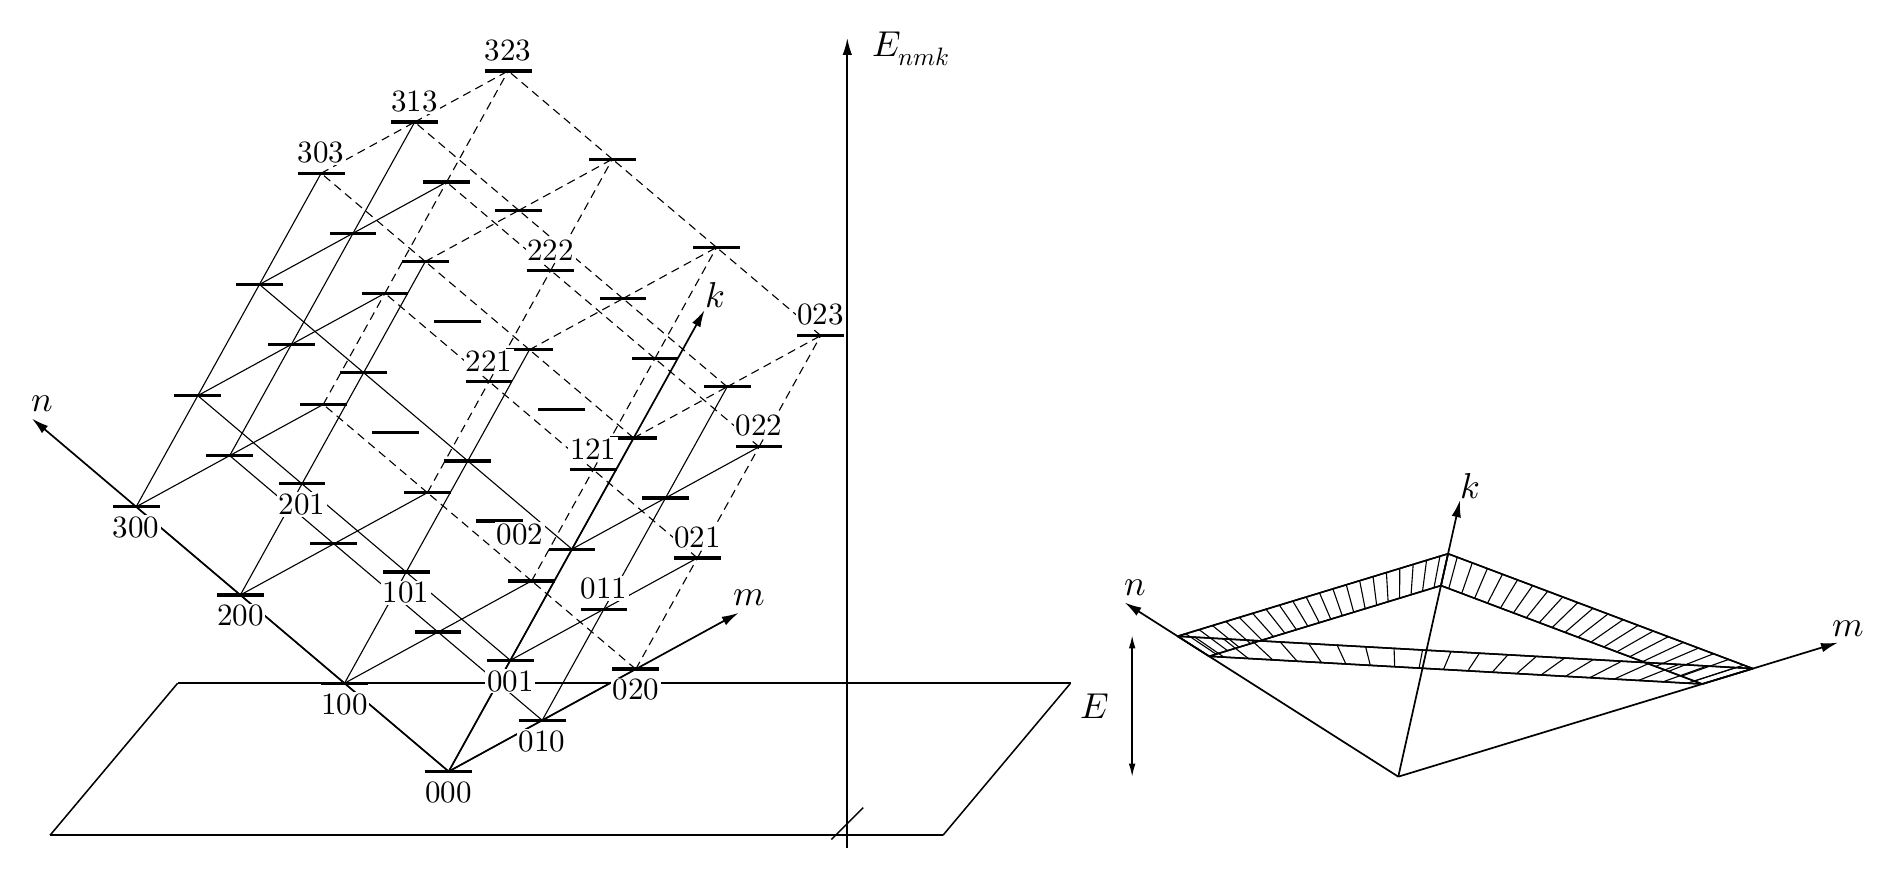
\begin{tikzpicture}[x=1cm,y=1cm,line join=round]
% CP15: Energy dimension begins on the bottom reference plane (0.48 cm),
% and reaches the lower surface of the unit-energy shell. The hatched shell
% is a schematic n,m,k projection, NOT a measured or exact molecular surface.
% The right-hand shell is shown in a second projection.
\begin{scope}[scale=1.35]
\draw[light] (3.400000,0.400000)--(2.420000,1.230000);
\draw[light] (3.400000,0.400000)--(4.280000,0.881400);
\draw[light] (3.400000,0.400000)--(3.980000,1.445800);
\draw[light] (3.980000,1.445800)--(3.000000,2.275800);
\draw[light] (3.980000,1.445800)--(4.860000,1.927200);
\draw[light] (3.980000,1.445800)--(4.560000,2.491600);
\draw[light] (4.560000,2.491600)--(3.580000,3.321600);
\draw[light] (4.560000,2.491600)--(5.440000,2.973000);
\draw[light] (4.560000,2.491600)--(5.140000,3.537400);
\draw[light,densely dashed] (5.140000,3.537400)--(4.160000,4.367400);
\draw[light,densely dashed] (5.140000,3.537400)--(6.020000,4.018800);
\draw[light] (4.280000,0.881400)--(3.300000,1.711400);
\draw[light] (4.280000,0.881400)--(5.160000,1.362800);
\draw[light] (4.280000,0.881400)--(4.860000,1.927200);
\draw[light] (4.860000,1.927200)--(5.740000,2.408600);
\draw[light] (4.860000,1.927200)--(5.440000,2.973000);
\draw[light] (5.440000,2.973000)--(6.320000,3.454400);
\draw[light] (5.440000,2.973000)--(6.020000,4.018800);
\draw[light,densely dashed] (6.020000,4.018800)--(5.040000,4.848800);
\draw[light,densely dashed] (6.020000,4.018800)--(6.900000,4.500200);
\draw[light,densely dashed] (5.160000,1.362800)--(4.180000,2.192800);
\draw[light,densely dashed] (5.160000,1.362800)--(5.740000,2.408600);
\draw[light,densely dashed] (5.740000,2.408600)--(4.760000,3.238600);
\draw[light,densely dashed] (5.740000,2.408600)--(6.320000,3.454400);
\draw[light,densely dashed] (6.320000,3.454400)--(5.340000,4.284400);
\draw[light,densely dashed] (6.320000,3.454400)--(6.900000,4.500200);
\draw[light,densely dashed] (6.900000,4.500200)--(5.920000,5.330200);
\draw[light] (2.420000,1.230000)--(1.440000,2.060000);
\draw[light] (2.420000,1.230000)--(3.300000,1.711400);
\draw[light] (2.420000,1.230000)--(3.000000,2.275800);
\draw[light] (3.000000,2.275800)--(2.020000,3.105800);
\draw[light] (3.000000,2.275800)--(3.580000,3.321600);
\draw[light] (3.580000,3.321600)--(2.600000,4.151600);
\draw[light] (3.580000,3.321600)--(4.160000,4.367400);
\draw[light,densely dashed] (4.160000,4.367400)--(3.180000,5.197400);
\draw[light,densely dashed] (4.160000,4.367400)--(5.040000,4.848800);
\draw[light] (3.300000,1.711400)--(2.320000,2.541400);
\draw[light] (3.300000,1.711400)--(4.180000,2.192800);
\draw[light,densely dashed] (5.040000,4.848800)--(4.060000,5.678800);
\draw[light,densely dashed] (5.040000,4.848800)--(5.920000,5.330200);
\draw[light,densely dashed] (4.180000,2.192800)--(3.200000,3.022800);
\draw[light,densely dashed] (4.180000,2.192800)--(4.760000,3.238600);
\draw[light,densely dashed] (4.760000,3.238600)--(3.780000,4.068600);
\draw[light,densely dashed] (4.760000,3.238600)--(5.340000,4.284400);
\draw[light,densely dashed] (5.340000,4.284400)--(4.360000,5.114400);
\draw[light,densely dashed] (5.340000,4.284400)--(5.920000,5.330200);
\draw[light,densely dashed] (5.920000,5.330200)--(4.940000,6.160200);
\draw[light] (1.440000,2.060000)--(0.460000,2.890000);
\draw[light] (1.440000,2.060000)--(2.320000,2.541400);
\draw[light] (1.440000,2.060000)--(2.020000,3.105800);
\draw[light] (2.020000,3.105800)--(1.040000,3.935800);
\draw[light] (2.020000,3.105800)--(2.600000,4.151600);
\draw[light] (2.600000,4.151600)--(1.620000,4.981600);
\draw[light] (2.600000,4.151600)--(3.180000,5.197400);
\draw[light,densely dashed] (3.180000,5.197400)--(2.200000,6.027400);
\draw[light,densely dashed] (3.180000,5.197400)--(4.060000,5.678800);
\draw[light] (2.320000,2.541400)--(1.340000,3.371400);
\draw[light] (2.320000,2.541400)--(3.200000,3.022800);
\draw[light,densely dashed] (4.060000,5.678800)--(3.080000,6.508800);
\draw[light,densely dashed] (4.060000,5.678800)--(4.940000,6.160200);
\draw[light,densely dashed] (3.200000,3.022800)--(2.220000,3.852800);
\draw[light,densely dashed] (3.200000,3.022800)--(3.780000,4.068600);
\draw[light,densely dashed] (3.780000,4.068600)--(2.800000,4.898600);
\draw[light,densely dashed] (3.780000,4.068600)--(4.360000,5.114400);
\draw[light,densely dashed] (4.360000,5.114400)--(3.380000,5.944400);
\draw[light,densely dashed] (4.360000,5.114400)--(4.940000,6.160200);
\draw[light,densely dashed] (4.940000,6.160200)--(3.960000,6.990200);
\draw[light] (0.460000,2.890000)--(1.340000,3.371400);
\draw[light] (0.460000,2.890000)--(1.040000,3.935800);
\draw[light] (1.040000,3.935800)--(1.920000,4.417200);
\draw[light] (1.040000,3.935800)--(1.620000,4.981600);
\draw[light] (1.620000,4.981600)--(2.500000,5.463000);
\draw[light] (1.620000,4.981600)--(2.200000,6.027400);
\draw[light,densely dashed] (2.200000,6.027400)--(3.080000,6.508800);
\draw[light] (1.340000,3.371400)--(2.220000,3.852800);
\draw[light] (1.340000,3.371400)--(1.920000,4.417200);
\draw[light] (1.920000,4.417200)--(2.800000,4.898600);
\draw[light] (1.920000,4.417200)--(2.500000,5.463000);
\draw[light] (2.500000,5.463000)--(3.380000,5.944400);
\draw[light] (2.500000,5.463000)--(3.080000,6.508800);
\draw[light,densely dashed] (3.080000,6.508800)--(3.960000,6.990200);
\draw[light,densely dashed] (2.220000,3.852800)--(2.800000,4.898600);
\draw[light,densely dashed] (2.800000,4.898600)--(3.380000,5.944400);
\draw[light,densely dashed] (3.380000,5.944400)--(3.960000,6.990200);
\draw[lev] (3.180000,0.400000)--(3.620000,0.400000);
\draw[lev] (3.760000,1.445800)--(4.200000,1.445800);
\draw[lev] (4.340000,2.491600)--(4.780000,2.491600);
\draw[lev] (4.920000,3.537400)--(5.360000,3.537400);
\draw[lev] (4.060000,0.881400)--(4.500000,0.881400);
\draw[lev] (4.640000,1.927200)--(5.080000,1.927200);
\draw[lev] (5.220000,2.973000)--(5.660000,2.973000);
\draw[lev] (5.800000,4.018800)--(6.240000,4.018800);
\draw[lev] (4.940000,1.362800)--(5.380000,1.362800);
\draw[lev] (5.520000,2.408600)--(5.960000,2.408600);
\draw[lev] (6.100000,3.454400)--(6.540000,3.454400);
\draw[lev] (6.680000,4.500200)--(7.120000,4.500200);
\draw[lev] (2.200000,1.230000)--(2.640000,1.230000);
\draw[lev] (2.780000,2.275800)--(3.220000,2.275800);
\draw[lev] (3.360000,3.321600)--(3.800000,3.321600);
\draw[lev] (3.940000,4.367400)--(4.380000,4.367400);
\draw[lev] (3.080000,1.711400)--(3.520000,1.711400);
\draw[lev] (3.660000,2.757200)--(4.100000,2.757200);
\draw[lev] (4.240000,3.803000)--(4.680000,3.803000);
\draw[lev] (4.820000,4.848800)--(5.260000,4.848800);
\draw[lev] (3.960000,2.192800)--(4.400000,2.192800);
\draw[lev] (4.540000,3.238600)--(4.980000,3.238600);
\draw[lev] (5.120000,4.284400)--(5.560000,4.284400);
\draw[lev] (5.700000,5.330200)--(6.140000,5.330200);
\draw[lev] (1.220000,2.060000)--(1.660000,2.060000);
\draw[lev] (1.800000,3.105800)--(2.240000,3.105800);
\draw[lev] (2.380000,4.151600)--(2.820000,4.151600);
\draw[lev] (2.960000,5.197400)--(3.400000,5.197400);
\draw[lev] (2.100000,2.541400)--(2.540000,2.541400);
\draw[lev] (2.680000,3.587200)--(3.120000,3.587200);
\draw[lev] (3.260000,4.633000)--(3.700000,4.633000);
\draw[lev] (3.840000,5.678800)--(4.280000,5.678800);
\draw[lev] (2.980000,3.022800)--(3.420000,3.022800);
\draw[lev] (3.560000,4.068600)--(4.000000,4.068600);
\draw[lev] (4.140000,5.114400)--(4.580000,5.114400);
\draw[lev] (4.720000,6.160200)--(5.160000,6.160200);
\draw[lev] (0.240000,2.890000)--(0.680000,2.890000);
\draw[lev] (0.820000,3.935800)--(1.260000,3.935800);
\draw[lev] (1.400000,4.981600)--(1.840000,4.981600);
\draw[lev] (1.980000,6.027400)--(2.420000,6.027400);
\draw[lev] (1.120000,3.371400)--(1.560000,3.371400);
\draw[lev] (1.700000,4.417200)--(2.140000,4.417200);
\draw[lev] (2.280000,5.463000)--(2.720000,5.463000);
\draw[lev] (2.860000,6.508800)--(3.300000,6.508800);
\draw[lev] (2.000000,3.852800)--(2.440000,3.852800);
\draw[lev] (2.580000,4.898600)--(3.020000,4.898600);
\draw[lev] (3.160000,5.944400)--(3.600000,5.944400);
\draw[lev] (3.740000,6.990200)--(4.180000,6.990200);
\draw[ax] (3.400000,0.400000)--(-0.520000,3.720000);
\node[lab] at (-0.420000,3.860000) {$n$};
\draw[ax] (3.400000,0.400000)--(6.128000,1.892340);
\node[lab] at (6.228000,2.032340) {$m$};
\draw[ax] (3.400000,0.400000)--(5.807000,4.740070);
\node[lab] at (5.907000,4.880070) {$k$};
\draw[fine] (-0.350000,-0.200000)--(8.050000,-0.200000);
\draw[fine] (-0.350000,-0.200000)--(0.850000,1.230000);
\draw[fine] (8.050000,-0.200000)--(9.250000,1.230000);
\draw[fine] (9.250000,1.230000)--(0.850000,1.230000);
\draw[ax] (7.150000,-0.320000)--(7.150000,7.300000);
\node[lab,anchor=west] at (7.340000,7.200000) {$E_{nmk}$};
\draw[fine] (7.000000,-0.240000)--(7.300000,0.060000);
\node[small,fill=white,inner sep=.6pt,anchor=north] at (3.400000,0.325000) {$000$};
\node[small,fill=white,inner sep=.6pt,anchor=north] at (2.420000,1.155000) {$100$};
\node[small,fill=white,inner sep=.6pt,anchor=north] at (1.440000,1.985000) {$200$};
\node[small,fill=white,inner sep=.6pt,anchor=north] at (0.460000,2.815000) {$300$};
\node[small,fill=white,inner sep=.6pt,anchor=north] at (3.980000,1.370800) {$001$};
\node[small,fill=white,inner sep=.6pt,anchor=east] at (4.310000,2.631600) {$002$};
\node[small,fill=white,inner sep=.6pt,anchor=north] at (4.280000,0.806400) {$010$};
\node[small,fill=white,inner sep=.6pt,anchor=south] at (4.860000,2.002200) {$011$};
\node[small,fill=white,inner sep=.6pt,anchor=north] at (5.160000,1.287800) {$020$};
\node[small,fill=white,inner sep=.6pt,anchor=south] at (5.740000,2.483600) {$021$};
\node[small,fill=white,inner sep=.6pt,anchor=south] at (6.320000,3.529400) {$022$};
\node[small,fill=white,inner sep=.6pt,anchor=south] at (6.900000,4.575200) {$023$};
\node[small,fill=white,inner sep=.6pt,anchor=north] at (2.020000,3.030800) {$201$};
\node[small,fill=white,inner sep=.6pt,anchor=north] at (3.000000,2.200800) {$101$};
\node[small,fill=white,inner sep=.6pt,anchor=south] at (4.760000,3.313600) {$121$};
\node[small,fill=white,inner sep=.6pt,anchor=south] at (3.780000,4.143600) {$221$};
\node[small,fill=white,inner sep=.6pt,anchor=south] at (4.360000,5.189400) {$222$};
\node[small,fill=white,inner sep=.6pt,anchor=south] at (2.200000,6.102400) {$303$};
\node[small,fill=white,inner sep=.6pt,anchor=south] at (3.080000,6.583800) {$313$};
\node[small,fill=white,inner sep=.6pt,anchor=south] at (3.960000,7.065200) {$323$};
\end{scope}
% CP15: enlarge the independent section diagram to author's right-hand panel share.
% All vertices and the three axis directions are preserved by one affine view transform.
\begin{scope}[shift={(-3.5cm,-.15cm)},scale=1.30]
\draw[ax] (15.500000,0.480000)--(12.826560,2.181280);
\node[lab] at (12.926560,2.321280) {$n$};
\draw[ax] (15.500000,0.480000)--(19.795103,1.789483);
\node[lab] at (19.895103,1.929483) {$m$};
\draw[ax] (15.500000,0.480000)--(16.102778,3.180444);
\node[lab] at (16.202778,3.320444) {$k$};
\draw[fine] (13.652000,1.656000)--(18.468966,1.385172)--(18.963793,1.536034)--(13.344000,1.852000) -- cycle;
\draw[light] (13.796509,1.647875)--(13.512594,1.842521);
\draw[light] (14.034822,1.634476)--(13.790626,1.826889);
\draw[light] (14.273135,1.621077)--(14.068658,1.811257);
\draw[light] (14.511448,1.607679)--(14.346689,1.795625);
\draw[light] (14.749761,1.594280)--(14.624721,1.779993);
\draw[light] (14.988074,1.580881)--(14.902753,1.764361);
\draw[light] (15.226387,1.567482)--(15.180785,1.748729);
\draw[light] (15.464700,1.554083)--(15.458817,1.733097);
\draw[light] (15.703013,1.540684)--(15.736849,1.717465);
\draw[light] (15.941326,1.527286)--(16.014881,1.701833);
\draw[light] (16.179639,1.513887)--(16.292912,1.686201);
\draw[light] (16.417952,1.500488)--(16.570944,1.670569);
\draw[light] (16.656265,1.487089)--(16.848976,1.654937);
\draw[light] (16.894578,1.473690)--(17.127008,1.639305);
\draw[light] (17.132891,1.460291)--(17.405040,1.623673);
\draw[light] (17.371204,1.446893)--(17.683072,1.608041);
\draw[light] (17.609517,1.433494)--(17.961104,1.592409);
\draw[light] (17.847830,1.420095)--(18.239136,1.576777);
\draw[light] (18.086144,1.406696)--(18.517167,1.561145);
\draw[light] (18.324457,1.393297)--(18.795199,1.545513);
\draw[fine] (18.468966,1.385172)--(15.916667,2.346667)--(15.986111,2.657778)--(18.963793,1.536034) -- cycle;
\draw[light] (18.392397,1.414017)--(18.874463,1.569687);
\draw[light] (18.266125,1.461586)--(18.727146,1.625184);
\draw[light] (18.139853,1.509155)--(18.579829,1.680680);
\draw[light] (18.013582,1.556723)--(18.432512,1.736177);
\draw[light] (17.887310,1.604292)--(18.285195,1.791674);
\draw[light] (17.761038,1.651861)--(18.137878,1.847171);
\draw[light] (17.634767,1.699429)--(17.990561,1.902667);
\draw[light] (17.508495,1.746998)--(17.843244,1.958164);
\draw[light] (17.382224,1.794567)--(17.695927,2.013661);
\draw[light] (17.255952,1.842135)--(17.548611,2.069158);
\draw[light] (17.129680,1.889704)--(17.401294,2.124655);
\draw[light] (17.003409,1.937273)--(17.253977,2.180151);
\draw[light] (16.877137,1.984841)--(17.106660,2.235648);
\draw[light] (16.750865,2.032410)--(16.959343,2.291145);
\draw[light] (16.624594,2.079979)--(16.812026,2.346642);
\draw[light] (16.498322,2.127547)--(16.664709,2.402138);
\draw[light] (16.372051,2.175116)--(16.517392,2.457635);
\draw[light] (16.245779,2.222685)--(16.370075,2.513132);
\draw[light] (16.119507,2.270253)--(16.222758,2.568629);
\draw[light] (15.993236,2.317822)--(16.075442,2.624125);
\draw[fine] (15.916667,2.346667)--(13.652000,1.656000)--(13.344000,1.852000)--(15.986111,2.657778) -- cycle;
\draw[light] (15.848727,2.325947)--(15.906848,2.633604);
\draw[light] (15.736685,2.291777)--(15.776133,2.593740);
\draw[light] (15.624644,2.257607)--(15.645418,2.553875);
\draw[light] (15.512602,2.223437)--(15.514703,2.514010);
\draw[light] (15.400561,2.189267)--(15.383988,2.474145);
\draw[light] (15.288520,2.155098)--(15.253273,2.434280);
\draw[light] (15.176478,2.120928)--(15.122558,2.394416);
\draw[light] (15.064437,2.086758)--(14.991843,2.354551);
\draw[light] (14.952395,2.052588)--(14.861128,2.314686);
\draw[light] (14.840354,2.018418)--(14.730413,2.274821);
\draw[light] (14.728313,1.984248)--(14.599698,2.234956);
\draw[light] (14.616271,1.950079)--(14.468983,2.195092);
\draw[light] (14.504230,1.915909)--(14.338268,2.155227);
\draw[light] (14.392188,1.881739)--(14.207553,2.115362);
\draw[light] (14.280147,1.847569)--(14.076838,2.075497);
\draw[light] (14.168106,1.813399)--(13.946123,2.035633);
\draw[light] (14.056064,1.779229)--(13.815408,1.995768);
\draw[light] (13.944023,1.745060)--(13.684693,1.955903);
\draw[light] (13.831981,1.710890)--(13.553978,1.916038);
\draw[light] (13.719940,1.676720)--(13.423263,1.876173);
\draw[fine] (13.652000,1.656000)--(18.468966,1.385172)--(15.916667,2.346667) -- cycle;
\draw[fine] (13.344000,1.852000)--(18.963793,1.536034)--(15.986111,2.657778) -- cycle;
\draw[dim] (12.900000,0.480000)--(12.900000,1.860000);
\node[lab,anchor=east] at (12.700000,1.170000) {$E$};

\end{scope}
\end{tikzpicture}
\end{document}
